%%%%%%%%%%%%%%%%%%%%%%%%%%%%%%%%%%%%%%%%%
%
% Space Physics
% Practical 2A
%
%%%%%%%%%%%%%%%%%%%%%%%%%%%%%%%%%%%%%%%%%

%----------------------------------------------------------------------------------------
%	DOCUMENT CONFIGURATIONS
%----------------------------------------------------------------------------------------

\documentclass{article}

\title{\textbf {Space Physics} \\ Practical 2A\\ Kinetic Theory} % Title
\def\authorivan{Ivan \v Sinkarenko}
\def\authoranu{Anuraj Rajendraprakash}
\author{\authorivan\\\authoranu}

\usepackage{graphicx}
\usepackage{fullpage}
\usepackage{url}
\usepackage{amsmath}

% load package with ``framed'' and ``numbered'' option.
\usepackage[framed,numbered,autolinebreaks,useliterate]{mcode}

\begin{document}

\maketitle % Insert the title, author and date

\centerline{Referee: Shahab Fatemi}

\setlength\parindent{0pt} % Removes all indentation from paragraphs

\renewcommand{\labelenumi}{\alph{enumi}.} % Make numbering in the enumerate environment by letter rather than number (e.g. section 6)
\clearpage

\clearpage

%----------------------------------------------------------------------------------------
%	SECTION 1. Discussion
%----------------------------------------------------------------------------------------

\section{Part II}
\subsection{Question 1}
Maxwellian distribution function was implemented using the following code:
\lstinputlisting{maxwellian.m}


\subsection{Question 2}
The code for this and the following question is as shown:
\lstinputlisting{question2.m}

The resulting plot is shown in Figure \ref{fig:plot2}. It represents the distribution function in linear and logarithmic scales. The most probable velocity is at 3 km/s which corresponds to the bulk velocity of the solar wind.
\begin{figure}[h!bt]
\centering
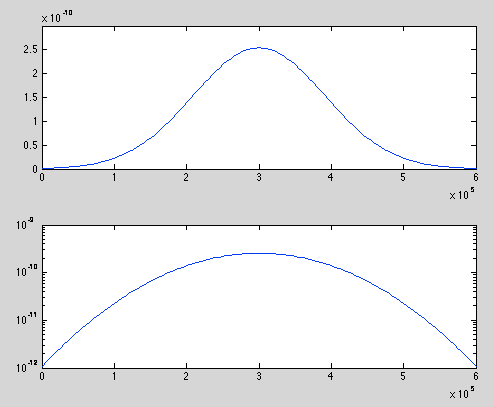
\includegraphics[width=0.7\textwidth]{Figures/plot_2.png}
\caption{Maxwellian distribution function.}
\label{fig:plot2}
\end{figure}

\subsection{Question 3}

From Figures \ref{fig:plot31} - \ref{fig:plot33} it is seen that the bigger gap $\Delta v$ we have, the less samples we take and consequently the distribution function gets more aliased.

\begin{figure}[h!tb]
\begin{minipage}[b]{0.33\linewidth}
\centering
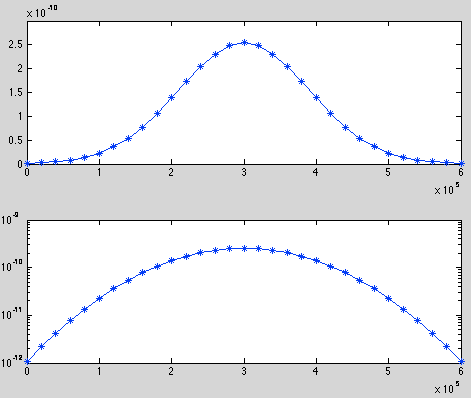
\includegraphics[width=\textwidth]{Figures/plot_31.png}
\caption{Distribution function with $\Delta v=2*10^4 m/s$}
\label{fig:plot31}
\end{minipage}
\begin{minipage}[b]{0.33\linewidth}
\centering
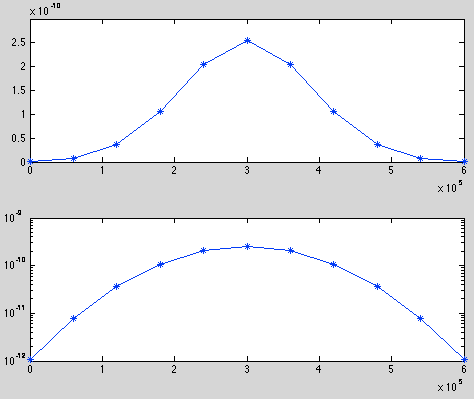
\includegraphics[width=\textwidth]{Figures/plot_32.png}
\caption{Distribution function with $\Delta v=6*10^4 m/s$}
\label{fig:plot32}
\end{minipage}
\begin{minipage}[b]{0.33\linewidth}
\centering
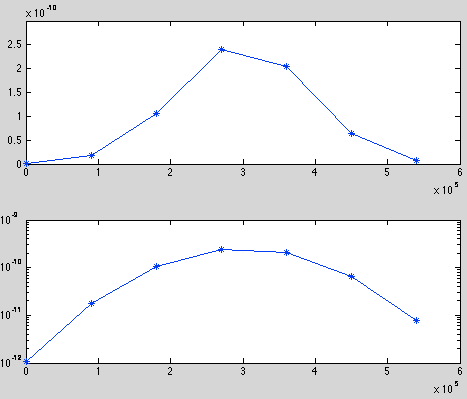
\includegraphics[width=\textwidth]{Figures/plot_33.png}
\caption{Distribution function with $\Delta v=9*10^4 m/s$}
\label{fig:plot33}
\end{minipage}
\end{figure}

\subsection{Question 4}

The 3D Maxwellian distribution function was found using the code:
\lstinputlisting{vsd_1.m}

\subsection{Question 5}
By running the above code we got following results:\\
\\
Initial solar wind density is: $8*10^6\:m^{-3}$, Computed number density is: $7.438228*10^6\:m^{-3}$ \\
Computation error is: $5.617717*10^5\:m^{-3}$\\
\\
The computed number density is almost the same, however it has an error about 7\%. This is due to kinetic temperature. The higher is temperature, the greater is the error.

\subsection{Question 6}
By changing the number density to $5*10^6$ and running the code we got following results:\\
\\
Initial solar wind density is: $5*10^6\:m^{-3}$, Computed number density is: $4.648893*10^6\:m^{-3}$\\
Computation error is: $3.511073*10^5\:m^{-3}$\\
\\
The error is still about 7\%.


\subsection{Question 7}
The plot in Figure \ref{fig:plot7} was done using \mcode{surf(v_x, v_y, f(:,:,ceil(length(v_z)/2))*1e11)} command;

\begin{figure}[h!bt]
\centering
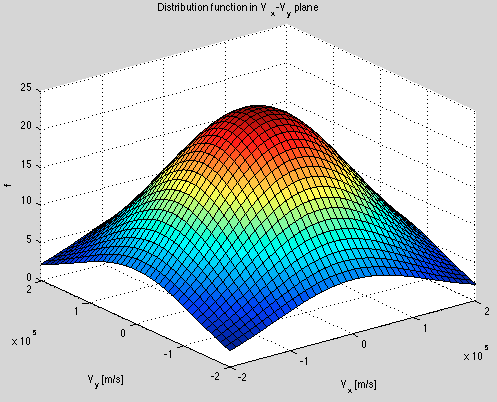
\includegraphics[width=0.5\textwidth]{Figures/plot_7.png}
\caption{3D Maxwellian distribution function.}
\label{fig:plot7}
\end{figure}

\subsection{Question 8}
The plot in Figure \ref{fig:plot8} was done using code:
\begin{lstlisting}
figure
subplot(1,2,1)
contour(v_x, v_y, f(:,:,ceil(length(v_z)/2)));
xlabel('V_y [m/s]')
ylabel('V_x [m/s]')
title('Contour map of the distribution function in V_x-V_y plane')
grid on
x = f(ceil(length(v_x)/2),:,:);
x = reshape(x,length(v_y),length(v_z));
subplot(1,2,2)
contour(v_y, v_z, f(:,:,ceil(length(v_x)/2)));
xlabel('V_z [m/s]')
ylabel('V_y [m/s]')
title('Contour map of the distribution function in V_y-V_z plane')
grid on
\end{lstlisting}
The distribution function is circular in both planes. It means that it is Maxwellian distribution function (Not Bi-Maxwellian).
\begin{figure}[h!bt]
\centering
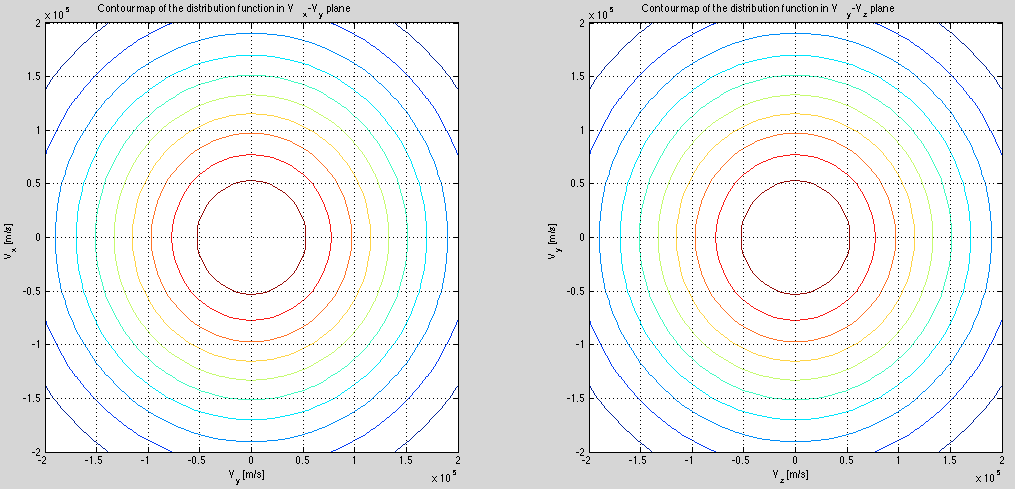
\includegraphics[width=\textwidth]{Figures/plot_8.png}
\caption{Contour of 3D Maxwellian distribution function in $v_x-v_y$ and $v_y-v_z$ planes.}
\label{fig:plot8}
\end{figure}

\subsection{Question 9}
For $T = 5*10^5 K$ the result is:\\
Initial solar wind density is: $8*10^6\:m^{-3}$, Computed number density is: $7.966393*10^6\:m^{-3}$\\
Computation error is: $3.360737*10^4\:m^{-3}$\\
\\
For $T = 20*10^5 K$ the result is:\\
Initial solar wind density is: $8*10^6\:m^{-3}$, Computed number density is: $5.629971*10^6\:m^{-3}$\\
Computation error is: $2.370029*10^6\:m^{-3}$\\
\\
Number density is significantly smaller when the kinetic temperature is greater.

\subsection{Question 10}
Group 2.

\subsection{Question 11}
\textbf{a)} Done using \mcode{load('group02.mat');} function.\\
\textbf{b)} The number density calculated using function \mcode{n = sum(f(:))*(dv^3)} is $2*10^6\:m^{-3}$.\\
\textbf{c)} The flux and solar wind bulk velocity (Gamma = [$-7.1999*10^{11}\:1.1036*10^{-5}\:-3.9621*10^4]$ $\:m^{-2}\:s^{-1}$, u\_sw = [$-3.6*10^5\:0\:0$] m/s) were calculated using code:
\begin{lstlisting}
[Gamma_x Gamma_y Gamma_z] = flux(v_x, v_y, v_z, dv, f)
u_sw = [Gamma_x/n Gamma_y/n Gamma_z/n]
\end{lstlisting}
\textbf{flux.m:}
\lstinputlisting{flux.m}
\textbf{d)} The contour plot of the distribution function in $v_x$-$v_y$ plane is shown in Figure \ref{fig:plot10d}. It is clearly seen that this function is centered at the coordinates of the solar wind velocity, that is, $-3.6*10^5$ on x-axis and 0 on y-axis.

\begin{figure}[h!tb]
\begin{minipage}[b]{0.33\linewidth}
\centering
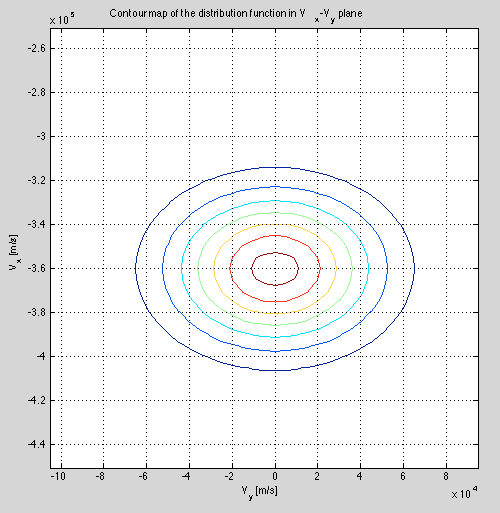
\includegraphics[width=\textwidth]{Figures/plot_10d.png}
\caption{Contour plot of the distribution function in $v_x$-$v_y$ plane.}
\label{fig:plot10d}
\end{minipage}
\begin{minipage}[b]{0.33\linewidth}
\centering
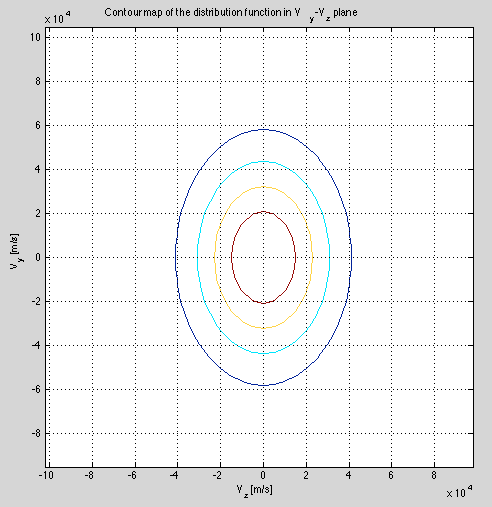
\includegraphics[width=\textwidth]{Figures/plot_10e1.png}
\caption{Contour plot of the distribution function in $v_y$-$v_z$ plane.}
\label{fig:plot10e1}
\end{minipage}
\begin{minipage}[b]{0.33\linewidth}
\centering
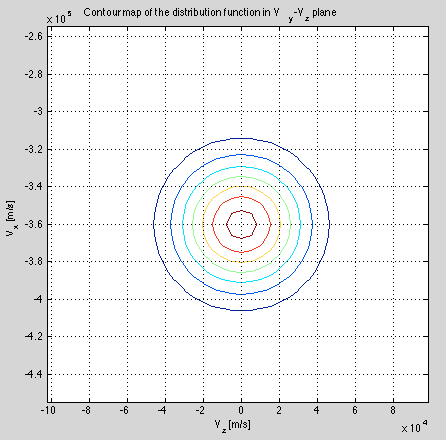
\includegraphics[width=\textwidth]{Figures/plot_10e2.png}
\caption{Contour plot of the distribution function in $v_x$-$v_z$ plane.}
\label{fig:plot10e2}
\end{minipage}
\end{figure}

\textbf{e)} This distribution function is Bi-Maxwellian because Figures \ref{fig:plot10d} and \ref{fig:plot10e1} have the plots which are eliptical, whereas the plot in Figure \ref{fig:plot10e2} is circular. It can be seen that the distribution function stretches out along y-axis. This is due to the magnetic field direction which has y-component and the distribution function is parallel to it.\\
\textbf{f)} The pressure tensor and the scalar pressure were calculated using the code:
\begin{lstlisting}
p_s = pressure_tensor(v_x, v_y, v_z, dv, f, u_sw, m)
scalar_p_s = trace(p_s)/3.0
\end{lstlisting}
\textbf{pressure\_tensor.m:}
\lstinputlisting{pressure_tensor.m}
Resulting values are: $P_s=\begin{bmatrix} 0.176*10^{-11} & 0 & 0 \\ 0 & 0.3521*10^{-11} & 0 \\ 0 & 0 & 0.176*10^{-11} \end{bmatrix};\:p_s = 2.3471*10^{-12}$.\\


\textbf{g)} The thermal velocity and solar wind kinetic temperature were calculated using the code:
\begin{lstlisting}
T = p_s /(n*k_b)
v_th = sqrt(2*k_b*T/m)
\end{lstlisting}
Resulting values are:\\
$T_s=\begin{bmatrix} 0.6375*10^5 & 0 & 0 \\ 0 & 1.275*10^5 & 0 \\ 0 & 0 & 0.6375*10^5 \end{bmatrix}\,K$\\
\\
\hspace{0.5cm}
\\
$v_{th} = \begin{bmatrix} 3.2441*10^4 & 0 & 0 \\ 0 & 4.5879*10^4 & 0 \\ 0 & 0 & 3.2441*10^4 \end{bmatrix}\,m/s$.\\
\end{document}